\documentclass[beamer,dvipsnames]{standalone}

\usepackage{tikz}
\usetikzlibrary{arrows}
\usetikzlibrary{positioning}
%\usetikzlibrary{positioning,decorations.pathreplacing,fit}
\usetikzlibrary{decorations.markings,arrows.meta}

\usepackage{bm}

\providecommand{\adlog}{\textcolor{red}{a}}
\providecommand{\bdlog}{\textcolor{blue}{b}}
\providecommand{\getsr}{\overset{\$}{\gets}}

\begin{document}

\begin{standaloneframe}

\resizebox{\textwidth}{!}{

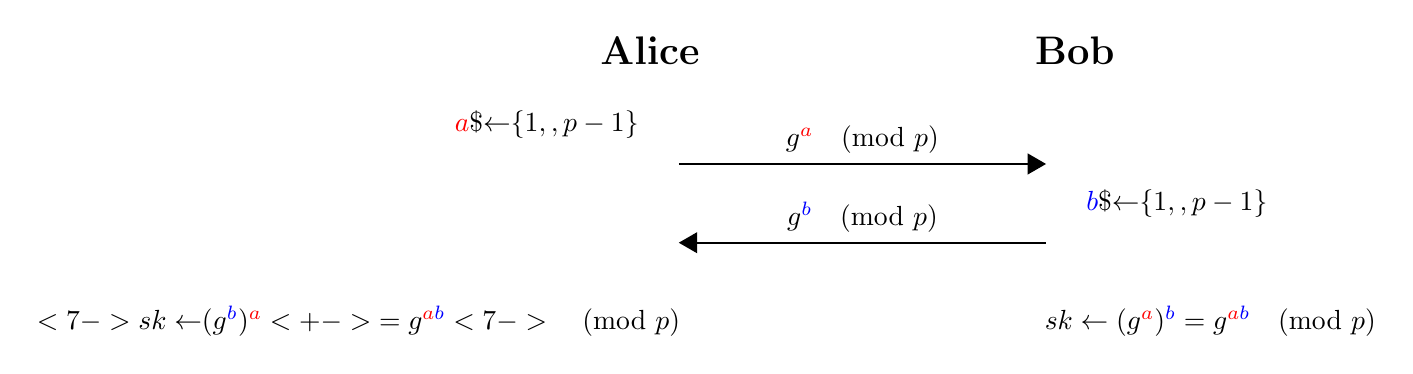
\begin{tikzpicture}[
		>=triangle 60,
	   	every path/.style={
	   		thick
	   	}
	]
	
	\node[] (client) {\Large\bfseries Alice};
	\node[right=4cm of client] (server) {\Large\bfseries Bob};
	

	\newcommand*{\MsgSpace}{0.5}
	\foreach \i in {1, ..., 6} {
		\node[below = \i * \MsgSpace of client,inner xsep=10pt] (c\i) {};
		\node[below = \i * \MsgSpace of server,inner xsep=10pt] (s\i) {};
	
	}



	\uncover<2->{
		\node[left=-10pt of c1] {$\adlog \getsr \lbrace 1, \dotsc, p-1 \rbrace$}; 
	}
	
	\uncover<3->{
		\draw[->] (c2.east) -- node[above] (M1) {$g^{\adlog} \pmod p$} (s2.west);
	}



	\uncover<5->{
		\node[right=-10pt of s3] {$\bdlog \getsr \lbrace 1, \dotsc, p-1 \rbrace$}; 
		\draw[<-] (c4.east) -- node[above] (M2) {$g^{\bdlog} \pmod p$} (s4.west);
	}
	

	\uncover<6->{
		\node[left=-25pt of c6] {$\uncover<7->{sk \gets} (g^{\bdlog})^{\adlog} \uncover<+->{= g^{\adlog\bdlog} \uncover<7->{\pmod p}}$}; 	
	}

	\uncover<8-16>{
		\node[right=-25pt of s6] {$sk \gets (g^{\adlog})^{\bdlog} = g^{\adlog\bdlog} \pmod p$}; 	
	}
		
	
\end{tikzpicture}

}

\end{standaloneframe}

\end{document}